\section{Methodology}
\label{sec:methodology}

In this section, we describe our methodology for the different analyses we perform with regard to leveraging on a PLF.
To be able to quantify the extent of leveraged positions over time, we first introduce a state transition framework for tracking the supply and borrow positions across all markets on a given PLF.
We then describe how we instantiate this framework on the Compound protocol using on-chain events data.

\subsection{Definitions}

Throughout the paper, we use the following definitions in the context of PLFs:

\begin{description}
\item[Market] A smart contract acting as the intermediary of loanable funds for a particular cryptoasset, where users supply and borrow funds. 

\item[Supply] Funds deposited to a market that can be loaned out to other users and used as collateral against depositors' own borrow positions.

\item[Borrow] Funds loaned out to users of a market.

\item[Collateral] Funds available to back a user's aggregate borrow positions.

\item[Locked funds] Funds remaining in the PLF smart contracts, equal to the difference between supplied and borrowed funds.

\item[Supplier] A user who deposits funds to a market.

\item[Borrower] A user who borrows funds from a market. Since a borrow position must be collateralized by deposited funds, a borrower must also be a supplier.

\item[Liquidator] A user who purchases a borrower's supply in a market when the borrower's collateral-to-borrow ratio falls below some threshold.
\end{description}


\subsection{States on a PLF}
In this section, we provide a formal definition of the state of a PLF.
We denote $\mathfrak{P}_t$ as the global state of a PLF at time $t$.
For brevity, in the following definitions, we assume that all the values are at a given time $t$.
We define the global state for the PLF as
\[
  \mathfrak{P} = (\mathcal{M},\Gamma, \mathcal{P}, \Lambda)
\]
where $\mathcal{M}$ is the set of states of individual markets, $\Gamma$ is the price the Oracle used, $\mathcal{P}$ is the set of states of individual participants and $\Lambda \in (0, 1)$ is the close factor of the protocol, which specifies the upper bound on the amount of collateral a liquidator may purchase.

We define the state of an individual market
$m \in \mathcal{M}$ as 
$$m = (\mathcal{I}, \mathcal{B}, \mathcal{S}, \mathcal{C})$$
where
$\mathcal{I}$ is the market's interest rate model,
$\mathcal{B}$ is the total borrows,
$\mathcal{S}$ is the total supply of deposits,
% $\mathcal{R}$ is the total reserves,
% $\mathcal{F}$ is the reserve factor,
and $\mathcal{C}$ is the collateral factor.
% ,
% and $\mathcal{P}_t^j$ the set of participants in market $m_t^j$.

$\mathcal{P}^m$ is the state of all participants in market $m$ and the positions of a participant $P$ in this market is defined as
\[
  P^m = (B^m,S^m)
\]
where $B^m$ and $S^m$ are respectively the total borrow positions and total supplied deposits of a market participant in market $m$.

For a given market $m$, the total deposits supplied $\mathcal{S}^m$ is thus given by:
\begin{equation}
    \mathcal{S}^m = \sum_{P^m\in \mathcal{P}^m} S^m
\end{equation}

Similarly, the market's total borrows $\mathcal{B}^m$ is given by:
\begin{equation}
    \mathcal{B}^m = \sum_{P^m\in \mathcal{P}^m} B^m
\end{equation}

The state of a participant $P$ is liquidable if the following holds: 
% \begin{equation}
%     \frac{\sum_{m\in \mathcal{M}}
%     \Big\{\left[S^{m} \cdot \mathcal{C} + \mathcal{I}(S^m)\right] \cdot \Gamma(m)\Big\}
%     }{
%     \sum_{m\in \mathcal{M}} \Big\{\left[B^m + \mathcal{I}(B^m)\right] \cdot \Gamma(m)\Big\}}
%     < \mathcal{K}
%     \label{eq:liqcond}
% \end{equation}

\begin{equation}
    \frac{\sum_{m\in \mathcal{M}}
    \Big\{\left[S^{m} \cdot \mathcal{C} + \mathcal{I}(S^m)\right] \cdot \Gamma(m) \cdot \mathcal{K}^m \Big\}
    }{
    \sum_{m\in \mathcal{M}} \Big\{\left[B^m + \mathcal{I}(B^m)\right] \cdot \Gamma(m)\Big\}}
    < 1
    \label{eq:liqcond}
\end{equation}
where $\Gamma(m)$ returns the price of the underlying asset denominated in a predefined numéraire (e.g. USD), $\mathcal{I}(S^m)$ returns the interest earned with supply $S^m$, $\mathcal{I}(B^m)$ returns the interest accrued with borrow $B^m$, and $\mathcal{K}^m \leq 1$ denotes the liquidation threshold of market $m$. In Compound, liquidation threshold $\mathcal{K}^m$ is set to be constant at 100\% protocol-wide, whereas with other protocols such as Aave, $\mathcal{K}^m$ is specific to the collateral asset from market $m$, and can be dynamically adjusted when the risk level of the asset changes. 


The transition from a state of a market $m$ from time $t$ to $t+1$ is given by some state transition $\sigma$, such that $m_{t}\xrightarrow[]{\sigma}m_{t+1}$. 

\subsection{Leveraging Spirals on a PLF}
\label{ssec:leveraging-spirals-meth}
Here we examine the workings of leveraging in DeFi using a PLF. 
We assume a speculator on some volatile asset $B$, holds initial capital $\alpha$ in $B$.
In order to increase his exposure to $B$, the speculator may borrow a stable asset $A$ against his $\alpha$ on a PLF at a collateralization ratio $\delta>1$.
For simplicity, we shall assume in this illustrative example that a speculator will leverage his position on the same PLF.
Note that the cost of borrowing is given by some floating interest rate $\gamma$ for the specific asset market.
In return for his collateral, the borrower receives $\frac{\alpha}{\delta}$ in the volatile asset $B$.
As the debt is denominated in units of a stable asset (e.g. \coin{DAI}), the borrower has an upper limit on his net debt, remaining unaffected by any volatility in the value of asset $A$.
In order to leverage his position, the debt denominated in $A$ may be used to buy\footnote{In practice this may be done via automated market makers \cite{xu2021dexAmm} (e.g. Uniswap~\cite{whitepaper:uniswap}) or via decentralized exchanges~\cite{web:dydx}.} additional units of asset $B$, which can subsequently be used to collateralize a new borrow position.
This process is illustrated in Figure~\ref{fig:plf-leverage} and can be repeated numerous times, by which the total exposure to asset $A$, the underlying collateral to the total debt in asset $A$, increases at a decaying rate.

% Explain how an agent can leverage a position in DeFi: this diagram is a draft
\begin{figure}[tbp]
    \centering
    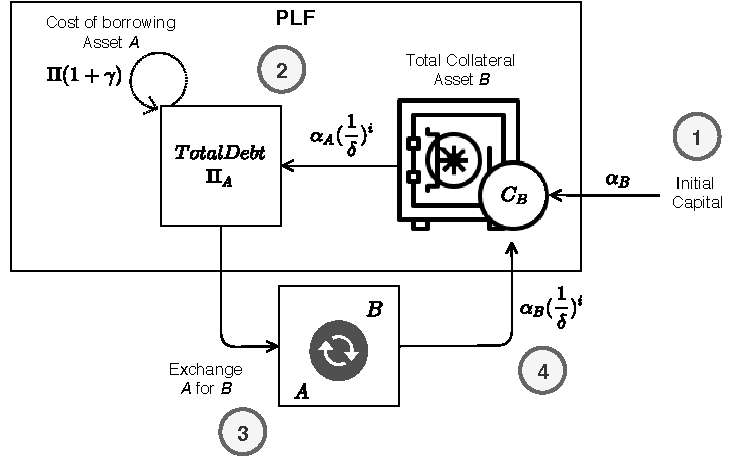
\includegraphics[width=0.8\textwidth]{6-application-security/figures/leveraging.pdf}
    \caption{The steps of leveraging using a PLF. \textbf{1.} Initial capital $\alpha_{B}$ in asset $B$ is deposited as collateral to borrow asset $A$. \textbf{2.} Interest accrues over the debt of the borrow position for asset $B$. \textbf{3.} The borrowed asset $A$ is sold for asset $B$ on the open market. \textbf{4.} The newly purchased units of asset $B$ are locked as collateral for a new borrow position of asset $A$.}
    \label{fig:plf-leverage}
\end{figure}

The total collateral $\mathcal{C}$ a borrower must post through a borrow position with a leverage factor $k$, a collateralization ratio $\delta$ and an initial capital amount $\alpha$ can be expressed as $\sum_{i=0}^{k}\frac{\alpha}{\delta^i}$.
Hence, the total debt $\Pi$ for the corresponding borrow position is:
\begin{equation}
    \Pi = \biggl(\sum_{i=1}^{k} \frac{\alpha}{\delta^i}\biggl) \cdot (1+\gamma)
    \label{eq:debt}
\end{equation}
where $\gamma$ is the interest rate.
Note that Equation~\eqref{eq:debt} assumes a borrower uses the same collateralization ratio $\delta$ for his positions, as well as that all debt is taken out for the same asset on the same PLF and hence the floating interest rate is shared across all borrow positions. 

% \subsection{Cost of Leveraging}


% \subsection{Use Cases of Leveraging in DeFi}
% We identify three main use cases for leveraging in DeFi:

% \point{Leveraged long position} To take on a long position of an asset refers to purchasing an asset with the expectation that it will appreciate in value. 
% In DeFi, such positions can be easily leveraged by locking the asset on which the long position shall be taken as collateral.

% \point{Leveraged short position}
% A short position refers to borrowing funds of an asset, which one believes will depreciate in value. 
% Consequently, the taker of a short position sells the borrowed asset, only to repurchase it and pay back the borrower once the price has fallen, while profiting from the price change of the shorted asset.
% This can be achieved by taking on a leveraged borrow position of a stablecoin, where the locked collateral is the asset to short.

% \point{Liquidity mining}
% As a means to attract liquidity, PLFs may distribute governance tokens to their liquidity providers.
% The way these tokens are distributed depends on the PLF. 
% For instance, on Compound, the governance token \coin{COMP}\footnote{Contract address: \contractaddr{0xc00e94cb662c3520282e6f5717214004a7f26888}} is distributed among users across markets proportionally to the total dollar value of funds borrowed and supplied.
% This directly incentivizes users to mine liquidity in a market through leveraging in order to receive a larger share of governance tokens.
% For example, a supplier of funds in market $A$ can borrow against his position additional funds of $A$, at the cost of paying the difference between the earned and paid interest. 
% The incentive for pursuing this behaviour exists if the reward (i.e. the governance token) exceeds the cost of borrowing.\point{Leveraged long position} To take on a long position of an asset refers to purchasing an asset with the expectation that it will appreciate in value. 
% In DeFi, such positions can be easily leveraged by locking the asset on which the long position shall be taken as collateral.







\subsection{States and the Compound PLF}
For our analysis, we apply our state transition framework to the Compound PLF.
Therefore, we briefly present the workings of Compound in the context of our framework.  


\begin{figure}[tb]
  \centering
  \scriptsize
  \setlength{\tabcolsep}{1.5pt}
  \begin{tabular}{lp{6cm}c}
    \toprule
    {\bf Event} & {\bf Description} &
    {\bf State variables affected}\\

    \midrule
    \texttt{Borrow}  & A new borrow position is created. & $\mathcal{B}$  \\ 
    \texttt{Mint} & cTokens are minted for new deposits. &  $\mathcal{S}$           \\
    \texttt{RepayBorrow} & A borrow position is partially/fully repaid.& $\mathcal{B}$            \\ 
    \texttt{LiquidateBorrow} & A borrow position is liquidated. & $\mathcal{B}$, $\mathcal{S}$             \\
    \texttt{Redeem} & cTokens are used to redeem deposits of the underlying asset. & $\mathcal{S}$ \\
    \texttt{NewCollateralFactor} & The collateral factor for the associated market is updated. & $\mathcal{C}$   \\
    \texttt{AccrueInterest} & Interest has accrued for the associated market and its borrow index is updated. & $\mathcal{B}$            \\
    \texttt{NewInterestRateModel} & The interest rate model for the associated market is updated. & $\mathcal{I}$             \\
    \texttt{NewInterestParams} & The parameters of the interest rate model for the associated market are updated. & $\mathcal{I}$            \\
    \texttt{NewCloseFactor} & The close factor is updated. &     $\Lambda$   \\
    % \texttt{MarketListed} & The associated market is now listed. & $\mathcal{M}$            \\
    % \texttt{MarketExited} & The associated market is no longer listed. & $\mathcal{M}$          \\
    % Add NewLiquidityIncentive?
    \bottomrule
  \end{tabular}
  \caption{The events emitted by the Compound protocol smart contracts used for initiating state transitions and the states affected by each event.}
\label{tab:compound-events}
\end{figure}


\point{State Transitions}
We initiate state transitions via events emitted from the Compound protocol smart contracts.
We provide an overview of the state variables affected by Compound events in \autoref{tab:compound-events}.
%An extensive list of all Compound events is given in Appendix~\ref{}.
% The majority of events that update the state of a market are emitted each time a market participant \textit{borrows}, \textit{supplies}, \textit{repays}, \textit{redeems} funds, or gets \textit{liquidated} in a market.
% A detailed list and description of all Compound events which we use as state transitions is given by Table~\ref{} in Appendix~\ref{}.

\point{Funds Supplied}
Every market on Compound has an associated ``cToken", a token that continuously appreciates against the underlying asset as interest accrues.
For every deposit in a market, a newly-minted amount of the market's associated cToken is transferred to the depositor.
Therefore, rather than tracking the total amount of the underlying asset supplied, we account the total deposits of an asset supplied by a market participant in the market's cTokens.
Likewise, we account the total supply of deposits in the market in cTokens.


\point{Funds Borrowed}
A borrower on Compound must use cTokens as collateral for his borrow position.
The borrowing capacity equals the current value of the supply multiplied by the collateral factor for the asset.
For example, given an exchange rate of 1~\coin{DAI}~=~50 \coin{cDAI}, a collateral factor of 0.75 for \coin{DAI} and a price of 1~\coin{DAI}~=~1~USD, a holder of 500 \coin{cDAI} (10 \coin{DAI}) would be permitted to borrow up to 7.5 USD worth of some other asset on Compound. 
Therefore, as funds are borrowed, an individual's total borrow position, as well as the respective market's total borrows are updated.

\point{Interest}
% Explain borrow index 
The accrual of interest is tracked per market via a borrow index, which corresponds to the total interest accrued in the market.
% We handle state transitions caused by borrow index updates through the \texttt{AccrueInterest} event.
The borrow index of a market is also used to determine and update the total debt of a borrower in the respective market.
When funds are borrowed, the current borrow index for the market is stored with the borrow position.
When additional funds are borrowed or repaid, the latest borrow index is used to compute the difference of accrued interest since the last borrow and added to the total debt.

\point{Liquidation}
A borrower on Compound is eligible for liquidation should his total supply of collateral, i.e. the value of the sum of the borrower's cToken holdings per market, weighted by each market's collateral factor, be less than the value of the borrower's aggregate debt (Equation~\eqref{eq:liqcond}).
The maximum amount of debt a liquidator may pay back in exchange for collateral is specified by the close factor of a market.
